\documentclass[12pt,a4paper,utf8x]{report}
\usepackage [frenchb]{babel}

% Pour pouvoir utiliser 
\usepackage{ucs}
\usepackage[utf8x]{inputenc}
\usepackage{graphicx}

\usepackage{url} % Pour avoir de belles url
\usepackage {geometry}

% Pour mettre du code source
\usepackage {listings}
% Pour pouvoir passer en paysage
\usepackage{lscape}

% Pour pouvoir faire plusieurs colonnes
\usepackage {multicol}
% Pour crééer un index
\usepackage{makeidx}
\makeindex

% Pour gérer les liens interractifs et les signets Acrobat
\usepackage{hyperref}
\hypersetup{
pdftitle={titre de mon document},
pdfauthor={Nom de l'auteur},
pdfsubject={Sujet du document},
pdfkeywords={les mots clefs},
bookmarks, % Création du signet
pdfstartview=FitH, % Page de la largeur de la fenêtre
colorlinks=true, % Liens en couleur
linkcolor=black, 	
anchorcolor=black, 	
citecolor=black, 	
filecolor=black, 	
menucolor=black,
runcolor=black,
urlcolor=black, 	
frenchlinks=black,
bookmarksnumbered=true, % Signet numéroté
pdfpagemode=UseOutlines, % Montre les bookmarks.
bookmarksopen =true,
}

% Pour afficher la bibliographie, mais pas nottoc (Table of Contents), notlof (List of Figures) ni notlot (List of Tables)
\usepackage[notlof, notlot]{tocbibind}


% Pour les entetes de page
% \usepackage{fancyheadings}
%\pagestyle{fancy}
%\renewcommand{\sectionmark}[1]{\markboth{#1}{}} 
%\renewcommand{\subsectionmark}[1]{\markright{#1}} 

% Pour l'interligne de 1.5
\usepackage {setspace}
% Pour les marges de la page
\geometry{a4paper, top=2.5cm, bottom=3.5cm, left=1.5cm, right=1.5cm, marginparwidth=1.2cm}

\parskip=5pt %% distance entre § (paragraphe)
\sloppy %% respecter toujours la marge de droite 

% Pour les pénalités :
\interfootnotelinepenalty=150 %note de bas de page
\widowpenalty=150 %% veuves et orphelines
\clubpenalty=150 

%Pour la longueur de l'indentation des paragraphes
\setlength{\parindent}{15mm}



%%%% debut macro pour enlever le nom chapitre %%%%
\makeatletter
\def\@makechapterhead#1{%
  \vspace*{50\p@}%
  {\parindent \z@ \raggedright \normalfont
    \interlinepenalty\@M
    \ifnum \c@secnumdepth >\m@ne
        \Huge\bfseries \thechapter\quad
    \fi
    \Huge \bfseries #1\par\nobreak
    \vskip 40\p@
  }}

\def\@makeschapterhead#1{%
  \vspace*{50\p@}%
  {\parindent \z@ \raggedright
    \normalfont
    \interlinepenalty\@M
    \Huge \bfseries  #1\par\nobreak
    \vskip 40\p@
  }}
\makeatother
%%%% fin macro %%%%

%Couverture 

\title
{
	\normalsize{Rapport HADL\\
	Université de Nantes\\
	2010-2011}\\
	\vspace{15mm}
	\Huge{Rapport HADL}
}
\author{DEJEAN Charles, POTTIER Vincent\\
	\vspace{45mm}
}


\begin{document}

\maketitle
%Remerciements

Je tiens à remercier :
et on met la liste des personnes que l'on remercie. Toto, tutu, titi. et on met la liste des personnes que l'on remercie. Toto, tutu, titi.et on met la liste des personnes que l'on remercie. Toto, tutu, titi.et on met la liste des personnes que l'on remercie. Toto, tutu, titi.


Et on met la liste des personnes que l'on remercie. Toto, tutu, titi.et on met la liste des personnes que l'on remercie. Toto, tutu, titi.et on met la liste des personnes que l'on remercie. Toto, tutu, titi.et on met la liste des personnes que l'on remercie. Toto, tutu, titi.et on met la liste des personnes que l'on remercie. Toto, tutu, titi.

%\clearpage

\tableofcontents
\clearpage

% Pour avoir un interligne de 1,5
\begin{onehalfspace}

\chapter{Introduction}


	
\clearpage


	

	




	









\chapter{Description du Méta-Modèle HADL : M2}

\section{Définition}

	Le Méta-Modèle HADL représente le language à composant que nous voulons developper. 
	Il doit contenir une représentation de tous les concepts permettant de faire fonctionner correctement une architecture à composant.
		
\section{Analyse}

Lorsque l'on regarde grossièrement un système basé sur une architecture à
composant, on remarque principalement 3 entités :
\begin{itemize}
	\item Des Liens, permettant la transmission des messages entre les différentes
	entités.
	\item Les Connecteurs, Entités adaptant les messages pour que les composants se
	comprennent.
	\item Les Composants, Entités métier de l'architecture.
\end{itemize}

\subsection{Les Liens}
	Les liens n'ont pas d'existence propre. Ce sont juste des relations
	unidirectionnelles qui lient deux éléments.
	
	Il en existe 2 types :
	\begin{itemize}
	\item Attachement : relie un connecteur via un de ses rôles et un composant via
	l'un de ses ports.
	\item Binding : relie une configuration via l'un de ses ports et l'un de ses
	composants internes via l'un de ses ports.
	\end{itemize}

\subsection{Les Connecteurs}
	Un Connecteur est une Entité qui reçoit un message venant d'un Composant et qui
	le modifie pour l'envoyer à un autre Composant, afin que celui-ci puisse le
	comprendre et l'utiliser.
	
	Pour cela un connecteur a besoin de plusieurs choses :
	\begin{itemize}
		\item Des Rôles : rôles ``From'' et rôles ``To''. Ce sont les points d'entrées et
		de sorties d'un message dans le Connecteur.
		\item Des Glues : c'est la partie métier du connecteur, qui modifie un
		message.
	\end{itemize}

\subsection{Les Composants}
	Il existe 2 types de composants : les Composants ``simples'', offrant par
	eux-mêmes des services, et les Configurations, qui sont composées de Composants
	et de Connecteurs.
	
	Tous les composants ont certains attributs en commun :
	\begin{itemize}
		\item Les Contraintes et les Propriétés : ce sont des éléments qui
		permettent d'ajouter des spécifications au composant.
		\item Les Services : la partie métier que fourni le composant.
	\end{itemize}
	
	\subsubsection{les Composants "simples"}
		Un composant ``simple'' est une Entité qui reçoit un message et qui va le
		traiter. Le message reçu peut contenir des données ou juste être un stimulus
		demandant au composant de s'activer. Afin de reçevoir un message et de pouvoir
		en envoyer, le composant a besoin de Ports sur lesquels des liens
		d'attachements ou des liens bindings vont venir se connecter.
		
	\subsubsection{les Configurations}
		Une Configuration est une Entité qui reçoit un message et qui, pour le
		traiter, va l'envoyer via un lien vers un des composants qu'elle contient.
		
		Ainsi une Configuration est composée de :
		\begin{itemize}
			\item Ports, permettant de reçevoir et d'envoyer des messages.
			\item Composants.
			\item Connecteurs.
			\item De lien d'attachement et de liens binding, pour tout faire communiquer
			en interne.
	\end{itemize}
		
\section{Diagrammes}

Voici comment se structure notre Méta-Modèle HADL. La notation ``From | To '',
au niveau des liens, montre qu'un lien peut partir d'un composant vers un
connecteur, et vice versa. En effet, cette subtilité est à noter, car nos liens
sont unidirectionnels.

	\begin{figure}[!h]
		\centering
		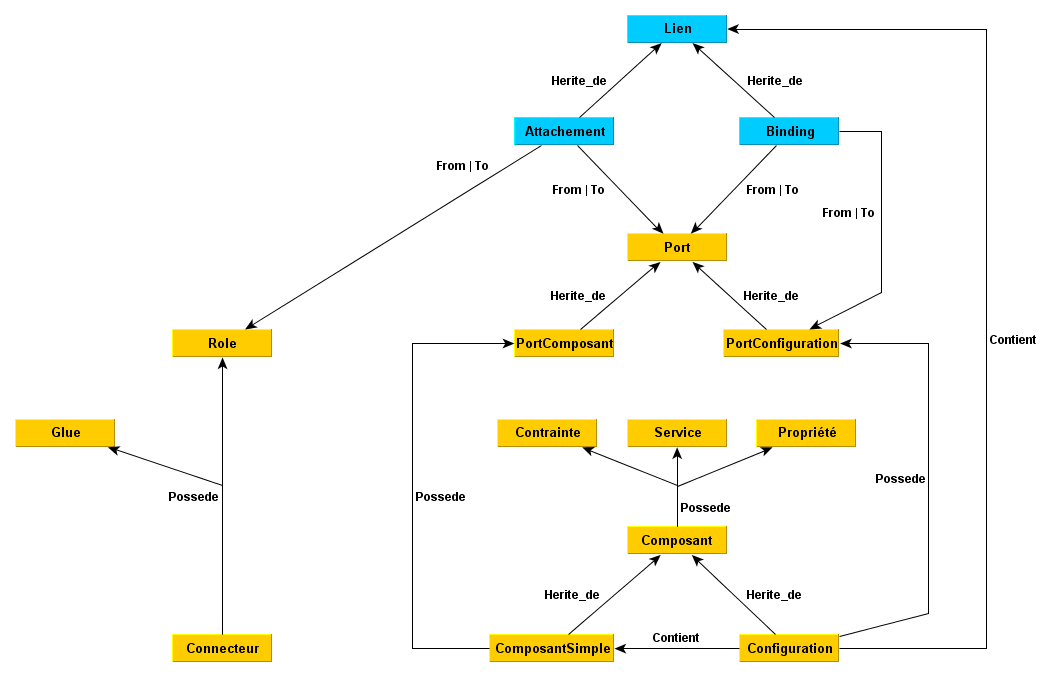
\includegraphics[scale=0.5]{../images/m2.PNG}
		\caption{représentation du M2}
	\end{figure}
		
\clearpage
\chapter{Description du système Client/Serveur : M1}
	
\section{Définition}
	Le système Client/Serveur que nous avons fabriqué à partir du Méta-Modèle HADL
	est très simple. Il est composé d'un client qui envoie une pseudo-requête SQL
	au serveur, qui lui répond.
	
	Le client est très basique. Il permet de saisir une requête, de l'envoyer et
	d'afficher la réponse.
	
	Le serveur lui est plus complexe. Il possède plusieurs fonctionnalités
	internes. Il vérifie que la requête est bien formée, que les éléments demandés
	et l'utilisateur existent et effectue la
	requete.

\section{Analyse}

	\subsection{Client/Serveur}
		C/S est notre système principal. C'est donc une Configuration qui va contenir: 
		\begin{itemize}
			\item le Composant Client.
			\item le Composant Serveur.
			\item le Connecteur RPC qui fait le pont entre Client et Serveur.
			\item un Port Configuration Start\_CS permettant d'activer le système.
			\item un Lien Binding reliant le Port Start\_CS au Client.
			\item plusieur Lien d'Attachement reliant le ClientS, le Serveur et RPC.
		\end{itemize}
		
	\subsection{Client}
		Le Client a un fonctionnement basique : saisi, envoie et reception. C'est
		donc un Composant "Simple". Nous lui fourniront 2 ports :
		\begin{itemize}
			\item Start : permet de lancer le client.
			\item Send-Request : permet d'envoyer un message vers le serveur et de
			recevoir sa réponse.
		\end{itemize}
		
	\subsection{Serveur}
		Le Serveur possède plusieurs fonctionnalités distinctes. C'est donc une
		Configuration va contenir :
		\begin{itemize}
			\item le Composant ConnectionManager : Composant qui gère la bonne syntaxe d'une requete.
			\item le Composant SecurityDB : Composant qui gère la vérification des droits utilisateur.
			\item le Composant DB : Composant contenant la base de données.
			\item le Connecteur ClearenceRequest : pont entre ConnectionManager et SecurityDB.
			\item le Connecteur SecurityQuery : pont entre SecurityDB et DB.
			\item le Connecteur SQLQuery : pont entre ConnectionManager et DB.
			\item Les Lien d'Attachements reliant tous les composants et connecteurs.
			\item Un Lien Binding reliant le Serveur au ConnectionManager.
			\end{itemize}
	
	\subsection{RPC}
		Le Connecteur RPC est très simple et permet de relier Le Client au Serveur.
		
		Il possède 4 rôles et 2 glues permettant de faire transiter un message du
		Client au Serveur et la réponse du Serveur au Client.

\section{Diagrammes}

Nous pouvons voir dans la figure \ref{m1} comment se structure notre système
Client/Serveur. Nous n'y avons pas affiché les attributs des différentes entités pour une meilleur lecture.

	\begin{figure}[!h]
		\centering
		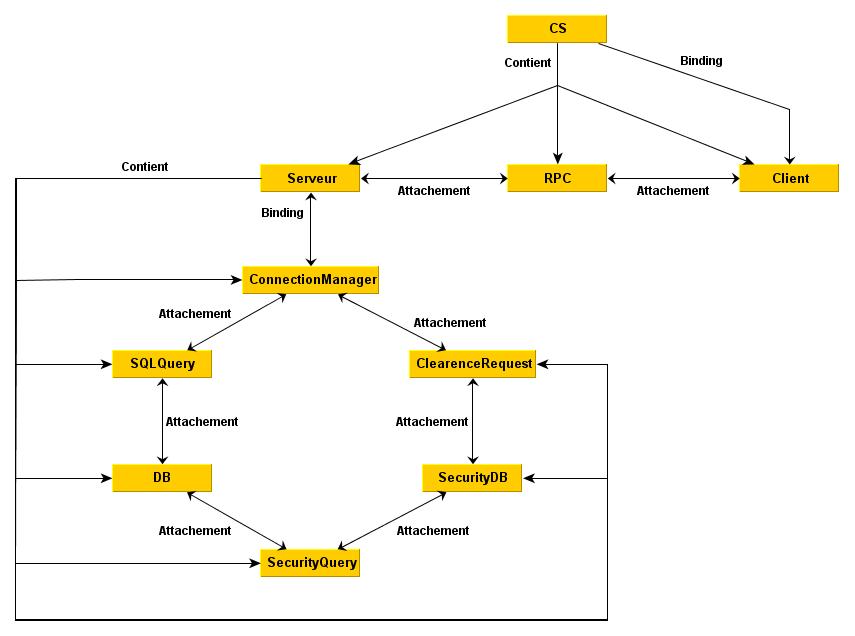
\includegraphics[scale=0.5]{../images/m1}
		\caption{représentation du M1}
		\label{m1}
	\end{figure}
	
Nous pouvons voir dans la figure \ref{zoom_m1} un zoom centré sur le composant
ConnectionManager, où les attributs sont affichés.

	\begin{figure}[!h]
		\centering
		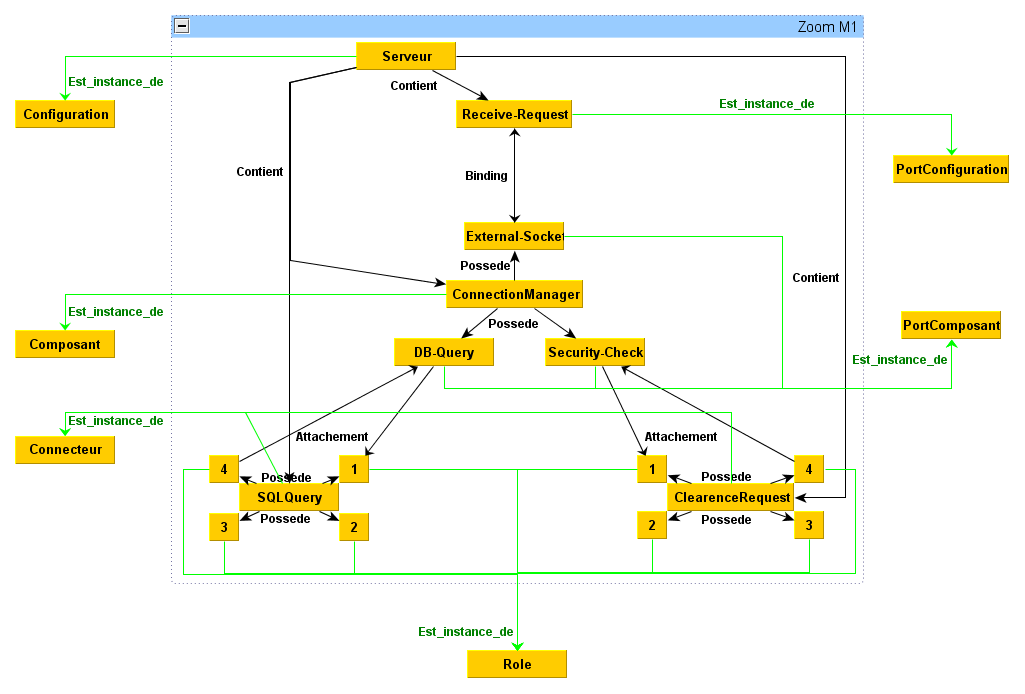
\includegraphics[scale=0.5]{../images/zoom_m1}
		\caption{zoom sur ConnectionManager}
		\label{zoom_m1}
	\end{figure}
	
\clearpage
\chapter{Description du Méta-Méta-Modèle Méta-HADL : M3}

	\section{Définition}
		
		Un Méta-Modèle permet à un modèle de s'auto-décrire. Il consiste à concevoir un modèle par lui même, à utiliser un modèle pour concevoir un autre modèle, à documenter un modèle et à comparer deux modèles.
		
	\section{Analyse}
		Afin de créer le Méta-HADL servant de base à notre HADL nous sommes partis du
		HADL et nous avons construit tous les éléments permettant de le définir
		correctement.
	
		\subsection{Meta-Entité}
			L'élément central servant de base à notre Meta-HADL et lui permettant de se redéfinir est Méta-Entité. A partir de cet élément nous allons tout construire.
			
			\begin{itemize}
				\item Relation : développée au paragraphe suivant.
				\item Entité : spécialisation d'une Méta-Entité.
				\item Attribut : Méta-Entité qui n'existe que pour appartenir à une autre
				Méta-Entité.
			\end{itemize}
		
		\subsection{Relation}
			Cet élément va permetre de définir les liens qui unissent les différents éléments :
				
			\begin{itemize}
				\item Est\_instance\_de : Spécialise une Méta-Entité en descendant d'un
				niveau dans les couches d'abstraction.
				\item Herite\_de : Spécialise une Méta-Entité en restant dans la même couche
				d'abstraction.
				\item Contient : Lie deux Méta-Entités en insérant l'une dans l'autre.
				\item Possede : Lie un Attribut à une Méta-Entité.
			\end{itemize}
			
			En plus de cela, elle possède deux attributs :
			\begin{itemize}
				\item From : Origine d'une relation.
				\item To : Destination d'une relation.
			\end{itemize}
			
	\section{Diagrammes}
	
		Voici comment se structure notre Méta-Méta-Modèle Méta-HADL.
	
		\begin{figure}[!h]
			\centering
			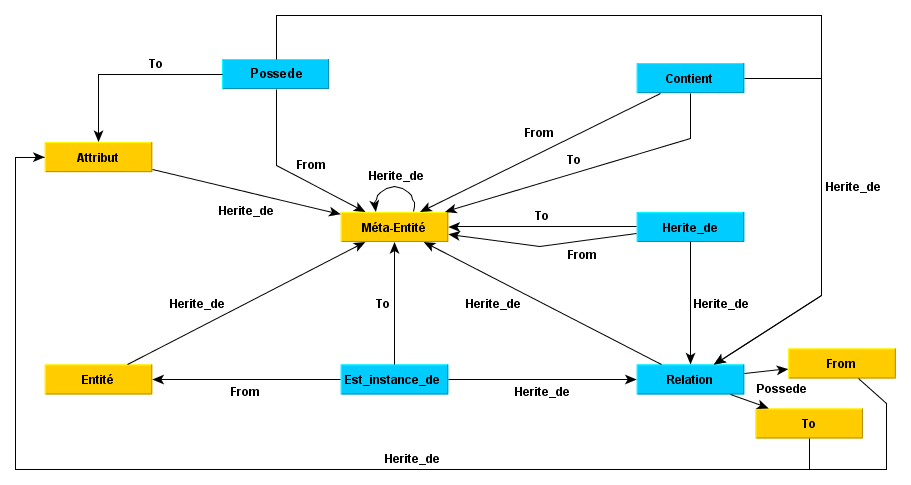
\includegraphics[scale=0.5]{../images/m3.png}
			\caption{représentation du M3}
		\end{figure}
	
\clearpage
\chapter{Vue générale}

	Voici une vue générale des différentes couches de notre architecture et des
	liens entre chaque couche.

	\begin{figure}[!h]
		\centering
		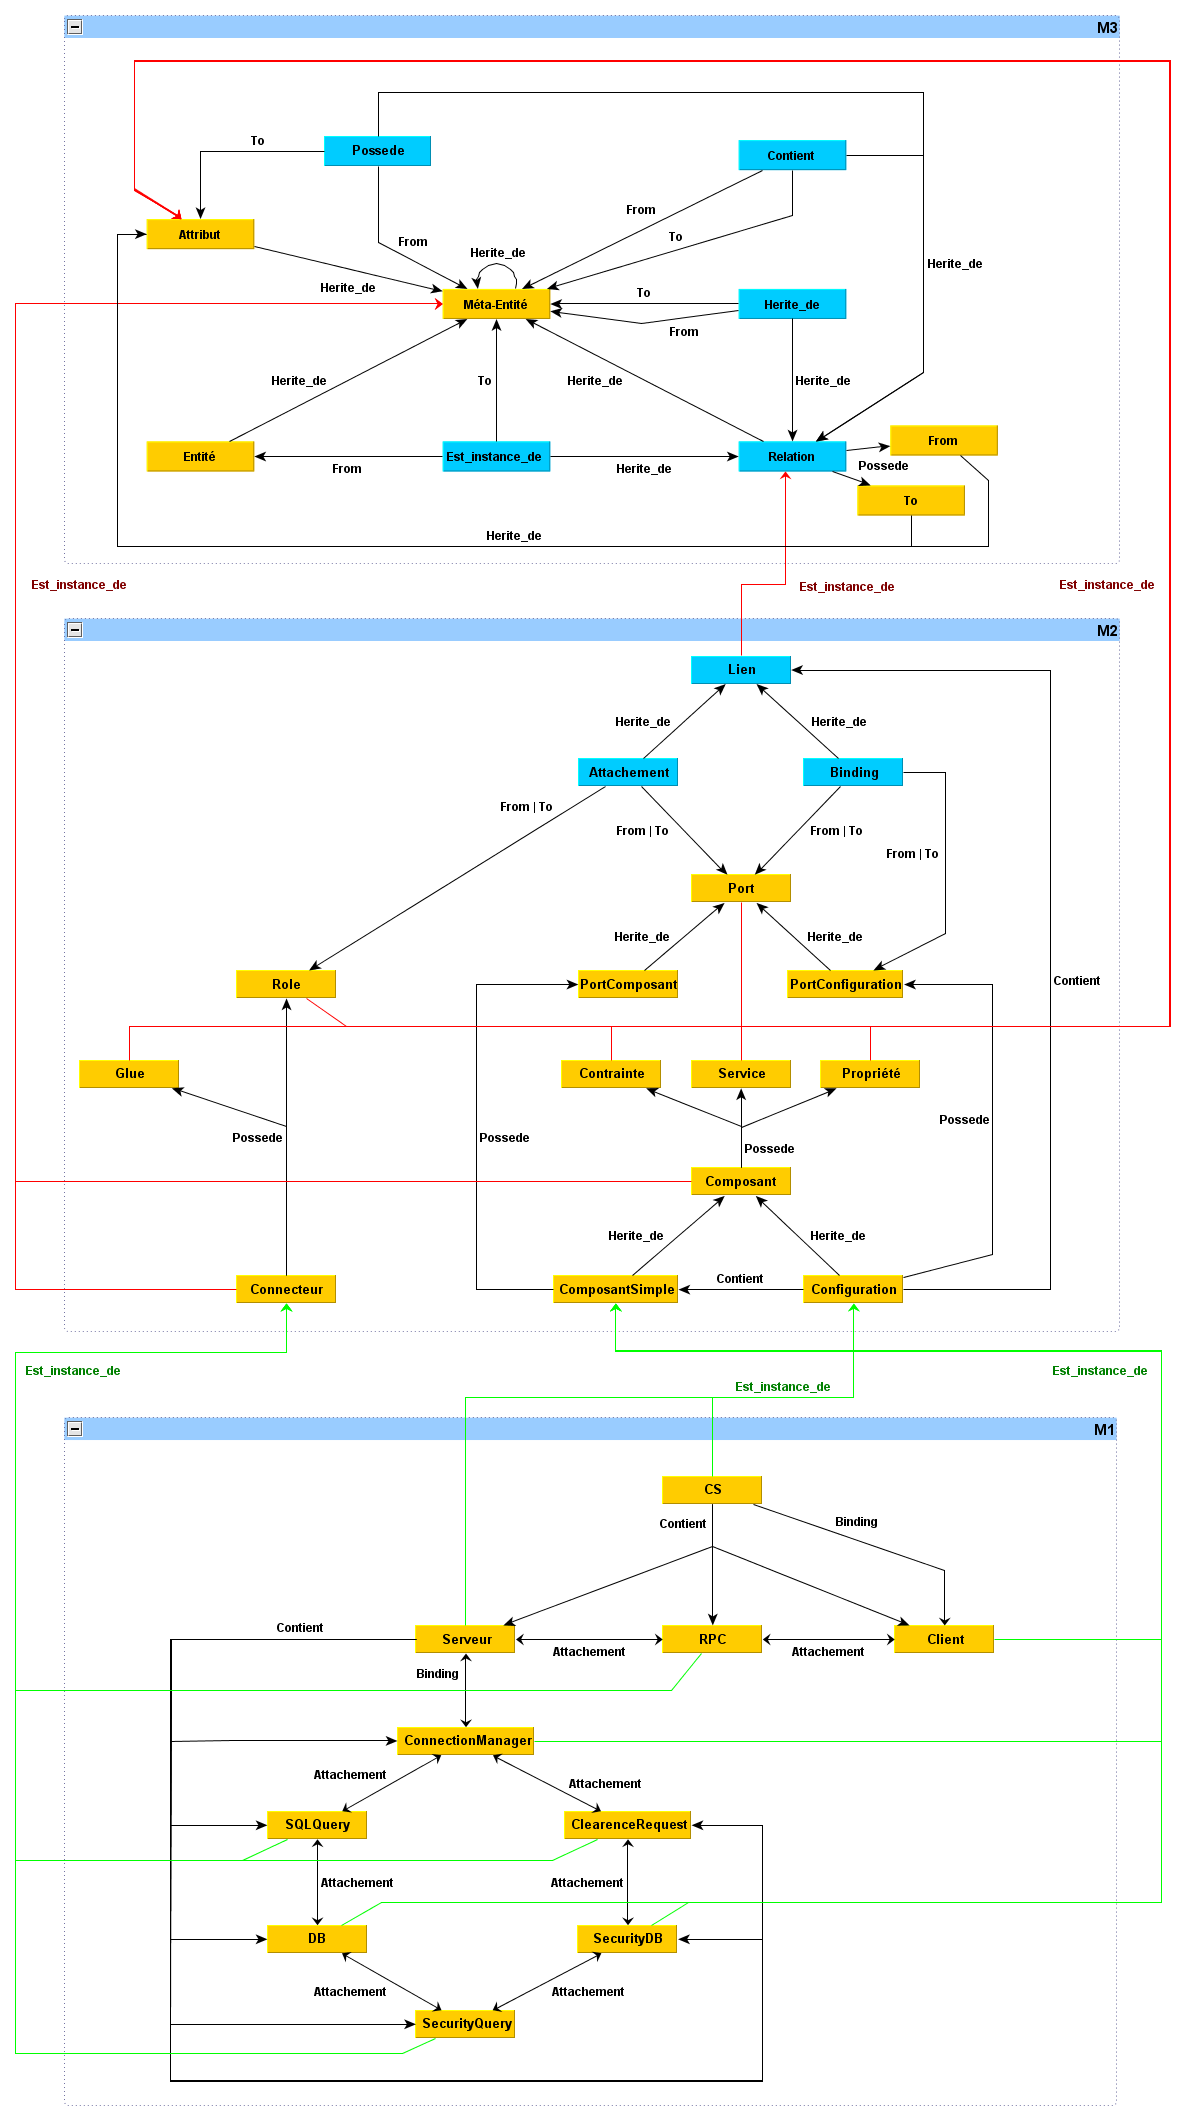
\includegraphics[scale=0.30]{../images/m.PNG}
	\end{figure}

\clearpage

% Pour finir l'interligne de 1,5
\end{onehalfspace}

%----------------------------------------
% Pour la bibliographie
%----------------------------------------
% Citer tous les ouvrages/références
% \nocite{*}
% Trier par ordre d'apparition
% \bibliographystyle{unsrt}
% Pour le style de la biblio
% \bibliographystyle{plain.bst}
% Ecrire la biblio ici
% \bibliography{biblio}

\printindex

\appendix


\end{document}
